\section{Simulation Validation}

% ════════════════════════════════════════════════════════════════
% SIMULATION SETUP
% ════════════════════════════════════════════════════════════════
\subsection{Simulation Setup}

\begin{frame}{\insertsubsectionhead}{}
  
  We employed the Lorenz system to validate the proposed method, as follows:
  \begin{equation}
    \ddtt
    \underbrace{
      \begin{pmatrix}
        x\\y\\z
      \end{pmatrix}
    }_{=:\mv{x}}
    =
    \underbrace{
      \begin{pmatrix}
        \sigma(y-x)
        \\
        x(\rho-z)-y
        \\
        xy-\beta z
      \end{pmatrix}
    }_{=:\mv{f}(\mv{x})}
    +
    \mysat
    \bigg(
      \underbrace{
        \begin{pmatrix}
            u_x\\u_y\\u_z
        \end{pmatrix}
      }_{=:\mv{u}}
    \bigg)
    +
    % \underbrace{
    %    \begin{pmatrix}
    %       d_x\\d_y\\d_z
    %    \end{pmatrix}
    % }_{=:\mv{d}}
    \mv{d}(t)
    ,
  \end{equation}
  where $\sigma=10$, $\rho=28$, and $\beta=8/3$.

  The saturation function and external disturbance are defined as follows:
  \begin{equation}
    \mysat(\mv{u})
    :=
    \begin{cases}
      \mv{u}
      ,
      & \text{if } \norm{\mv{u}} \le \overline{u}
      ,
      \\
      \overline{u} \tfrac{\mv{u}}{\norm{\mv{u}}}
      ,
      & \text{otherwise}
      ,
    \end{cases}
    ,
    \quad
    \text{and}
    \quad
    \mv{d}(t)
    :=
    1000 (H(t-0.1)-H(t-0.11))
    \cdot
    \mv{1}_{3\times1}
    ,
  \end{equation}
  where $\overline{u}=160$ and $H(\cdot)$ is the Heaviside step function.

  The desired trajectory is given by simulating the system with desired control law defined as follows:
  \begin{equation}
    \mv{u}_d(t)
    :=
    -\mv{f}(\mv{x}_d(t))
    -2(\mv{x}_d(t)-\mv{r})
    ,
    \text{ where }
    \mv{r} =
    \begin{pmatrix}
      -8.485\\8.485\\27
    \end{pmatrix}
    .
  \end{equation}

\end{frame}
% ————————————————————————————————————————————————————————————————

% ════════════════════════════════════════════════════════════════
% SIMULATION RESULTS
% ════════════════════════════════════════════════════════════════
\subsection{Simulation Results}

\begin{frame}{\insertsubsectionhead}{}
  
  \begin{columns}
  
    \column{0.5\textwidth}     

    \begin{table}[t]
      \renewcommand{\arraystretch}{1.3}
      \caption{Controllers for comparative study.}
      \centering
      % \begin{tabular}{c m{13.5em}}
      \begin{tabular}{l}
      \hline 
      \hline 
      (C$_1$) \protect\colorLine{blue}{solid}  
      Proposed controller. \\ 
      \hline
      (C$_2$) \protect\colorLine{my_cyan}{solid} 
      CV-STEM (\cite{Tsukamoto:2021ae}). \\
      \hline
      (C$_3$) \protect\colorLine{gray}{solid} \\ 
      Desired controller for nominal model, \ie $\mv{u}=\mv{u}_d$. \\
      \hline
      \end{tabular}
      \label{table:controllers}
    \end{table}

    \column{0.5\textwidth}     

    \begin{figure}[t]
      \centering
      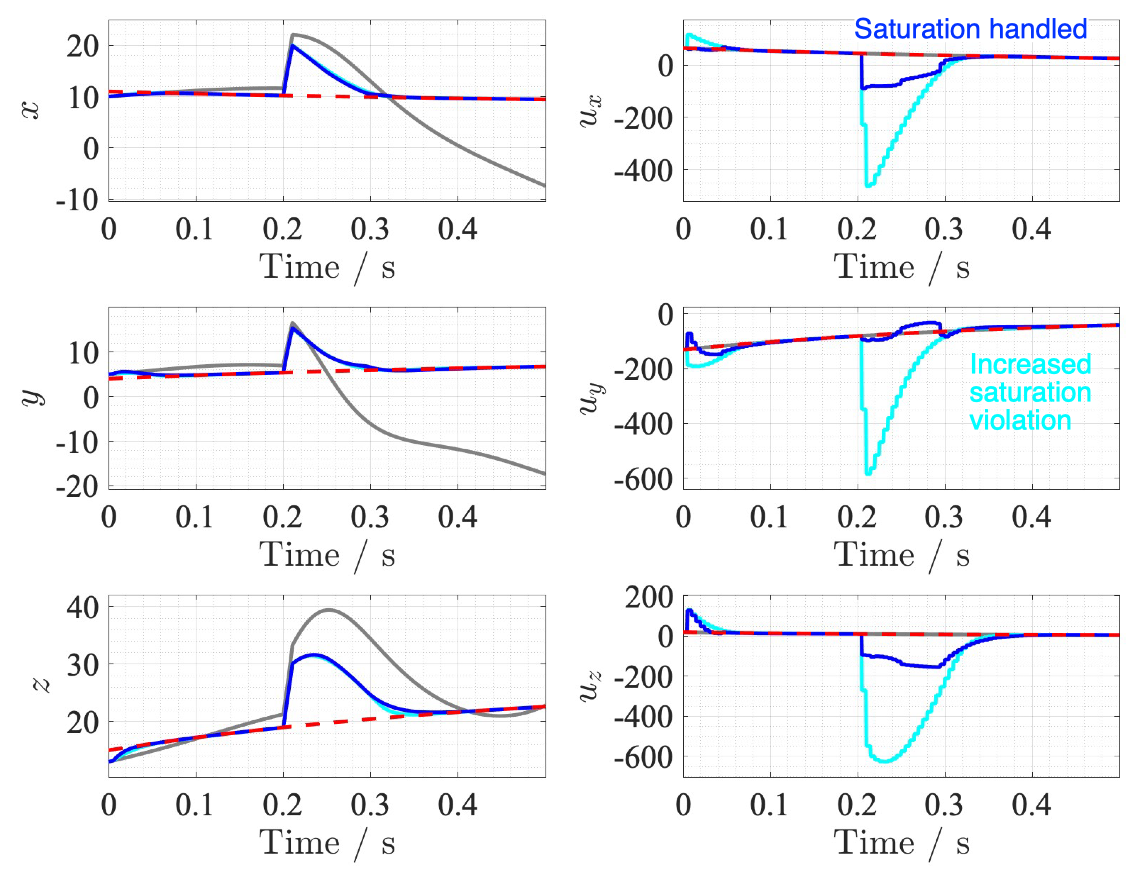
\includegraphics[width=0.99\linewidth]
      {
        figures/compare/main_fig1.png
      }
      \caption{
        Trajectories tracking results and control inputs
      }
    \end{figure}
  
  \end{columns}

\end{frame}
% ————————————————————————————————————————————————————————————————